\documentclass[a4paper,14pt]{extreport}
	\usepackage[left=1.5cm,right=1.5cm,
	    top=1.5cm,bottom=2cm,bindingoffset=0cm]{geometry}
	\usepackage{scrextend}
	\usepackage[T1,T2A]{fontenc}
	\usepackage[utf8]{inputenc}
	\usepackage[english,russian,ukrainian]{babel}
	\usepackage{tabularx}
	\usepackage{pgfplots}
	\usepackage{amssymb}
	\linespread{1.5}
	\usepackage{color}
	\usepackage{amsmath}
	\usepackage{mathrsfs}
	\usepackage{listings}
	\usepackage{graphicx}
	\graphicspath{ {./images/} }
	\usepackage{lipsum}
	\usepackage{xcolor}
	\usepackage{hyperref}
	\usepackage{tcolorbox}
	\usepackage{tikz}
	\usepackage[framemethod=TikZ]{mdframed}
	\usepackage{wrapfig,boxedminipage,lipsum}
	\mdfdefinestyle{MyFrame}{%
	linecolor=blue,outerlinewidth=2pt,roundcorner=20pt,innertopmargin=\baselineskip,innerbottommargin=\baselineskip,innerrightmargin=20pt,innerleftmargin=20pt,backgroundcolor=gray!50!white}
	 \usepackage{csvsimple}
	 \usepackage{supertabular}
	\usepackage{pdflscape}
	\usepackage{fancyvrb}
	%\usepackage{comment}
	\usepackage{array,tabularx}
	\usepackage{colortbl}
	\usepackage{fp}

	\usepackage{varwidth}
	\tcbuselibrary{skins}
	\usepackage{fancybox}


	\usepackage{tikz}
	\usepackage[framemethod=TikZ]{mdframed}
	\usepackage{xcolor}
	\usetikzlibrary{calc}
	\makeatletter
	\newlength{\mylength}
	\xdef\CircleFactor{1.1}
	\setlength\mylength{\dimexpr\f@size pt}
	\newsavebox{\mybox}
	\newcommand*\circled[2][draw=blue]{\savebox\mybox{\vbox{\vphantom{WL1/}#1}}\setlength\mylength{\dimexpr\CircleFactor\dimexpr\ht\mybox+\dp\mybox\relax\relax}\tikzset{mystyle/.style={circle,#1,minimum height={\mylength}}}
	\tikz[baseline=(char.base)]
	\node[mystyle] (char) {#2};}
	\makeatother

	\definecolor{ggreen}{rgb}{0.4,1,0}
	\definecolor{rred}{rgb}{1,0.1,0.1}
	\definecolor{amber}{rgb}{1.0, 0.75, 0.0}
	\definecolor{babyblue}{rgb}{0.54, 0.81, 0.94}
	\definecolor{amethyst}{rgb}{0.6, 0.4, 0.8}

	\usepackage{float}
	\usepackage{wrapfig}
	\usepackage{framed}
	%for nice Code{
	\lstdefinestyle{customc}{
	  belowcaptionskip=1\baselineskip,
	  breaklines=true,
	  frame=L,
	  xleftmargin=\parindent,
	  language=C,
	  showstringspaces=false,
	  basicstyle=\small\ttfamily,
	  keywordstyle=\bfseries\color{green!40!black},
	  commentstyle=\itshape\color{purple!40!black},
	  identifierstyle=\color{blue},
	  stringstyle=\color{orange},
	}
	\lstset{escapechar=@,style=customc}
%}


\begin{document}
\pagecolor{white}

%----------------------------------------1
\newtcbox{\xmybox}[1][red]{on line, arc=7pt,colback=#1!10!white,colframe=#1!50!black, before upper={\rule[-3pt]{0pt}{10pt}},boxrule=1pt, boxsep=0pt,left=6pt,right=6pt,top=2pt,bottom=2pt}



\begin{titlepage}
	\begin{center}
	\large
	Національний технічний університет України \\ "Київський політехнічний інститут імені Ігоря Сікорського"


	Факультет Електроніки

	Кафедра мікроелектроніки
	\vfill

	\textsc{ЗВІТ}\\

	{\Large Про виконання лабораторної роботи №3\\
	з дисципліни: «Твердотільна електроніки-1»\\[1cm]

	«Дослідження поверхні напівпровідника методом вольт-фарадних характеристик МДН-структури» \\

	}
	\bigskip
	\end{center}
	\vfill

	\newlength{\ML}
	\settowidth{\ML}{«\underline{\hspace{0.4cm}}» \underline{\hspace{2cm}}}
	\hfill
	\begin{minipage}{1\textwidth}
	Виконавець:\\
	Студент 3-го курсу \hspace{4cm} $\underset{\text{(підпис)}}{\underline{\hspace{0.2\textwidth}}}$  \hspace{1cm}А.\,С.~Мнацаканов\\
	\vspace{1cm}

	Перевірив: \hspace{6.1cm} $\underset{\text{(підпис)}}{\underline{\hspace{0.2\textwidth}}}$  \hspace{1cm}Л.\,М.~Королевич\\

	\end{minipage}

	\vfill

	\begin{center}
	2021
	\end{center}
\end{titlepage}
%---------------------------------------------------------------------------------------------------------------------------------------------------------------------------------
\newpage
\setcounter{page}{2}



\begin{center}1. МЕТА РОБОТИ\\ \end{center}

Дослідження величини, природи та стабільності заряду поверхневих
станів напівпровідника з допомогою вольт-фарадних характеристик ємності
структури метал-діелектрик-напівпровідник (МДН).

\begin{center}2. ЗАВДАННЯ\\ \end{center}

	1. Скласти схему для вимірювання ємності МДН-структури.\\

	2. Виконати вимірювання вольт-фарадної характеристики – залежності 
	ємності конденсатора МДН-структури від напруги зміщення. Діапазон напруг 
	від -20 В до +20 В. Частота вимірювального сигналу 1...2 МГц.\\

	3. Провести «вольт-температурні (В-Т) випробування» МДН-структури 
	при додатній та (або) при від’ємній полярностях постійної напруги., 
	прикладеної під час витримки при високій температурі.\\

	4. Побудувати зняті графіки вольт-фарадних (В-Ф) характеристик на 
	одному малюнку.\\

	5. Визначити за видом знятої вольт-фарадної характеристики тип 
	провідності напівпровідникової основи мікросхеми.\\

	6. Розрахувати із первинної В-Ф-характеристики величину, густину та 
	полярність заряду поверхневих станів.\\

	7. Розрахувати зміну заряду після «В-Т-випробувань» і пояснити природу 
	походження та причину нестабільності заряду поверхневих станів в 
	дослідженій МДН структури.



\newpage
\begin{center}2.1. СХЕМА ДОСЛІДЖЕННЯ\\ \end{center}

\begin{figure}[h]
\center{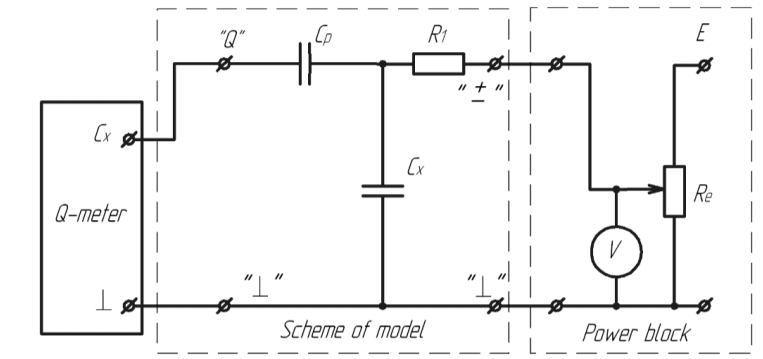
\includegraphics[width=0.8\linewidth]{1.png}}
\caption{Електрична схема установки дослідження вольт-фарадних 
характеристик}
\label{ris1}
\end{figure}




\clearpage
\begin{center}2.2.Таблиці\\ \end{center}
	\begin{minipage}{0.9\textwidth}
	\begin{center}
	Табл. 1 Вимірювання Вольт-Фарадних характеристик МДН-структури
	Умови вимірювань: $C_0$=370пФ; $F_0$=1,44МГц; $S_{\text{мдн}}$=1 мм$^2$. $\triangle C$ = 0,1 пФ; $\triangle U$ = 5 мВ. $\varepsilon$ = 3.9
	\end{center}
		\begin{minipage}{0.4\textwidth}
			\begin{tabular}{|c|c|c|}
			\hline
			C1    & Uz,B   & Cмдн, пФ \\ \hline
			262,7 & 0      & 107,3    \\ \hline
			262,9 & -1,01 & 107,1    \\ \hline
			263,5 & -1,99 & 106,5    \\ \hline
			263,6 & -2,5   & 106,4    \\ \hline
			265   & -3     & 105      \\ \hline
			264,7 & -3,55  & 105,3    \\ \hline
			265,2 & -3,78  & 104,8    \\ \hline
			266,1 & -4     & 103,9    \\ \hline
			266,9 & -4,2   & 103,1    \\ \hline
			27015 & -4,15   & 99,5      \\ \hline
			273,2 & -4,7   & 96,8     \\ \hline
			274,5 & -4,8   & 95,5     \\ \hline
			275,2 & -4,9   & 94,8     \\ \hline
			277   & -5,09  & 93       \\ \hline
			277,6 & -5,1  & 92,4     \\ \hline
			278,4 & -5,4  & 91,6     \\ \hline
			279,2 & -5,7   & 90,8     \\ \hline
			279,9 & -6     & 90,1     \\ \hline
			280,1 & -6,2   & 89,9     \\ \hline
			280,1 & -6,4   & 89,9     \\ \hline
			\end{tabular}
		\end{minipage}
		\hfill
		\begin{minipage}{0.4\textwidth}
			\begin{tabular}{|l|l|l|}
			\hline
			C1    & Uz,B   & Cмдн, пФ \\ \hline
			258,2 & 0      & 111,8    \\ \hline
			258,4 & -0,98 & 111,6    \\ \hline
			258,6 & -1,97 & 111,4    \\ \hline
			258,7 & -2,31 & 111,3    \\ \hline
			259   & -2,69 & 111      \\ \hline
			259,4 & -3,1 & 110,6    \\ \hline
			260,1 & -3,40 & 109,9    \\ \hline
			260,9 & -3,61 & 109,1    \\ \hline
			262,5 & -3,9 & 107,5    \\ \hline
			266,8 & -4,3 & 103,2    \\ \hline
			271,6 & -4,7 & 98,4     \\ \hline
			273,6 & -4,9   & 96,4     \\ \hline
			275,3 & -5,19  & 94,7     \\ \hline
			276,6 & -5,41  & 93,4     \\ \hline
			277   & -5,6   & 93       \\ \hline
			277,9 & -6     & 92,1     \\ \hline
			278,5 & -6,5   & 91,5     \\ \hline
			278,5 & -6,7   & 91,5     \\ \hline
			278,6 & -7     & 91,4     \\ \hline
			278,6 & -7,3   & 91,4     \\ \hline
			\end{tabular}
		\end{minipage}
\end{minipage}


%---------------------------------------------------------------------------------------------------------------------------------------------------------------------------------

\newpage
\begin{center}3.Графіки\\ \end{center}
	Будую сімейство використовуючи дані з Таб.1.
	\begin{center}
	\begin{tikzpicture}
		\begin{axis}[table/col sep = semicolon,
			title=Вольт-фарадні характеристик,
			xlabel = {$U_z$, В},
			ylabel = {$C_{\text{мдн}}$, пФ},
			height = 0.5\paperheight, 
			width = 0.5\paperwidth,
			/pgf/number format/1000 sep={}]
		\addplot table [grid style = both, x={b}, y={c}] {1.csv};
		\addplot table [grid style = both, x={f}, y={g}] {1.csv};
		\end{axis}		
	\end{tikzpicture}
\end{center}

\begin{center}
Головні значення
\end{center}

\begin{minipage}{0.4\textwidth}
  - $C_{d} \approx 110$ пФ\\

- $\dfrac{C_{\max }}{C_{\min }}\approx 0,8$\\

- $N_{a(d)}\approx 5 \cdot 10^{17} \text{см}^{3}$\\

- $C_{f b} \approx 0,9$ пФ\\
\end{minipage}
\hfill
\begin{minipage}{0.4\textwidth}
 - $U_{f b}\approx \pm 4 \mathrm{~B}$\\

- $U_{s s}\approx\pm 3 \mathrm{~B}$\\

- $Q_{s s}=U_{s s} \cdot M_{\text {мдн }}\approx 4 \cdot 10^{-10}$ Кл\\

- $N_{s s}\approx25 \cdot 10^{11} \text{ см}^{2}$\\
\end{minipage}






\clearpage
\begin{center}4. Висновок\\ \end{center}
	В даній лабораторній роботі було досліджено ємності структури МДН за допомогою отриманих вольт-фарадних характеристик. Якзо проаналізувати отримані результати, то можена побачити, що два зразки відрізняються 
	лише концентрацією домішок, але виходячи з теоретичних відомостей це саме той прараметр, що може вплинути на всі інші величини які не були розраховані.




\end{document}
